Con el objetivo de conocer todas las tareas necesarias para desarrollar el proyecto para posteriormente estimar su duración y planificarlas correctamente es necesario realizar una Estructura de Desglose del Trabajo (o WBS\footnote{El concepto de \textit{Work Breakdown Structure} fue introducido durante el desarrollo de la Técnica de Revisión y Evaluación de Programas (PERT) por el Departamento de Defensa de los Estados Unidos.  El WBS permite conocer todas las tareas necesarias para desarrollar un proyecto.  Para más información se recomienda consultar el capítulo 5 del PMBOK \cite{pmi:pmbok}}).

A continuación se mostrarán los diversos diagramas de la Estructura de Desglose del Trabajo.  Por su tamaño los diagramas se han subdividido para facilitar su lectura.  El orden en el que se relacionan los diagramas es el siguiente:
\begin{enumerate}
	\item
		La figura \ref{fig:wbs_analisis} muestra el diagrama de la fase de análisis del sistema, que produce como resultado la especificación formal del sistema a desarrollar.
	\item
		Posteriormente, la figura \ref{fig:wbs_diseno} muestra el diagrama de la fase del diseño de sistema, que produce como resultado el diseño de la arquitectura del sistema, de sus componentes y el modelo de datos final.
	\item
		Una vez obtenido el diseño, la figura \ref{fig:wbs_CMS} muestra el diagrama de las tareas pertenecientes al desarrollo del gestor de contenidos y sus módulos.  Por su tamaño, las tareas pertenecientes al desarrollo de la zona social se han dividido en un diagrama diferente (figura \ref{fig:wbs_social}).
	\item
		En paralelo al desarrollo del gestor de contenidos y sus módulos podría tener lugar el desarrollo del Punto de Entrada de Datos al portal, cuyo diagrama de tareas se muestra en la figura \ref{fig:wbs_datos}.
	\item
		Una vez desarrollados los componentes del sistema tendrían lugar las fases de integración y pruebas de aceptación.  El diagrama de tareas de ésta fase se muestra en al figura \ref{fig:wbs_final}.
\end{enumerate}

\begin{figure}[h]
	\centering
	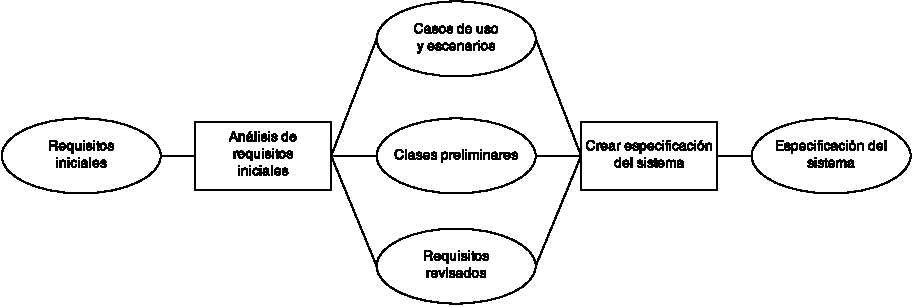
\includegraphics[width=\textwidth]{wbs/wbs_analisis}
	\caption{Estructura de desglose del trabajo de la fase de análisis del sistema}
	\label{fig:wbs_analisis}
\end{figure}

\begin{figure}[h]
	\centering
	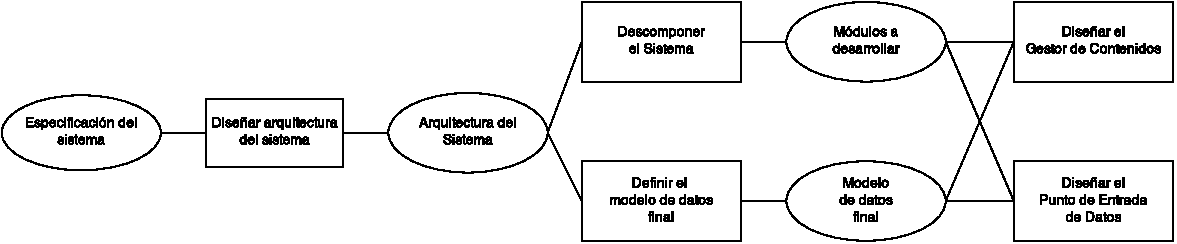
\includegraphics[width=\textwidth]{wbs/wbs_diseno}
	\caption{Estructura de desglose del trabajo de la fase de diseño del sistema}
	\label{fig:wbs_diseno}
\end{figure}

\begin{figure}[h]
	\centering
	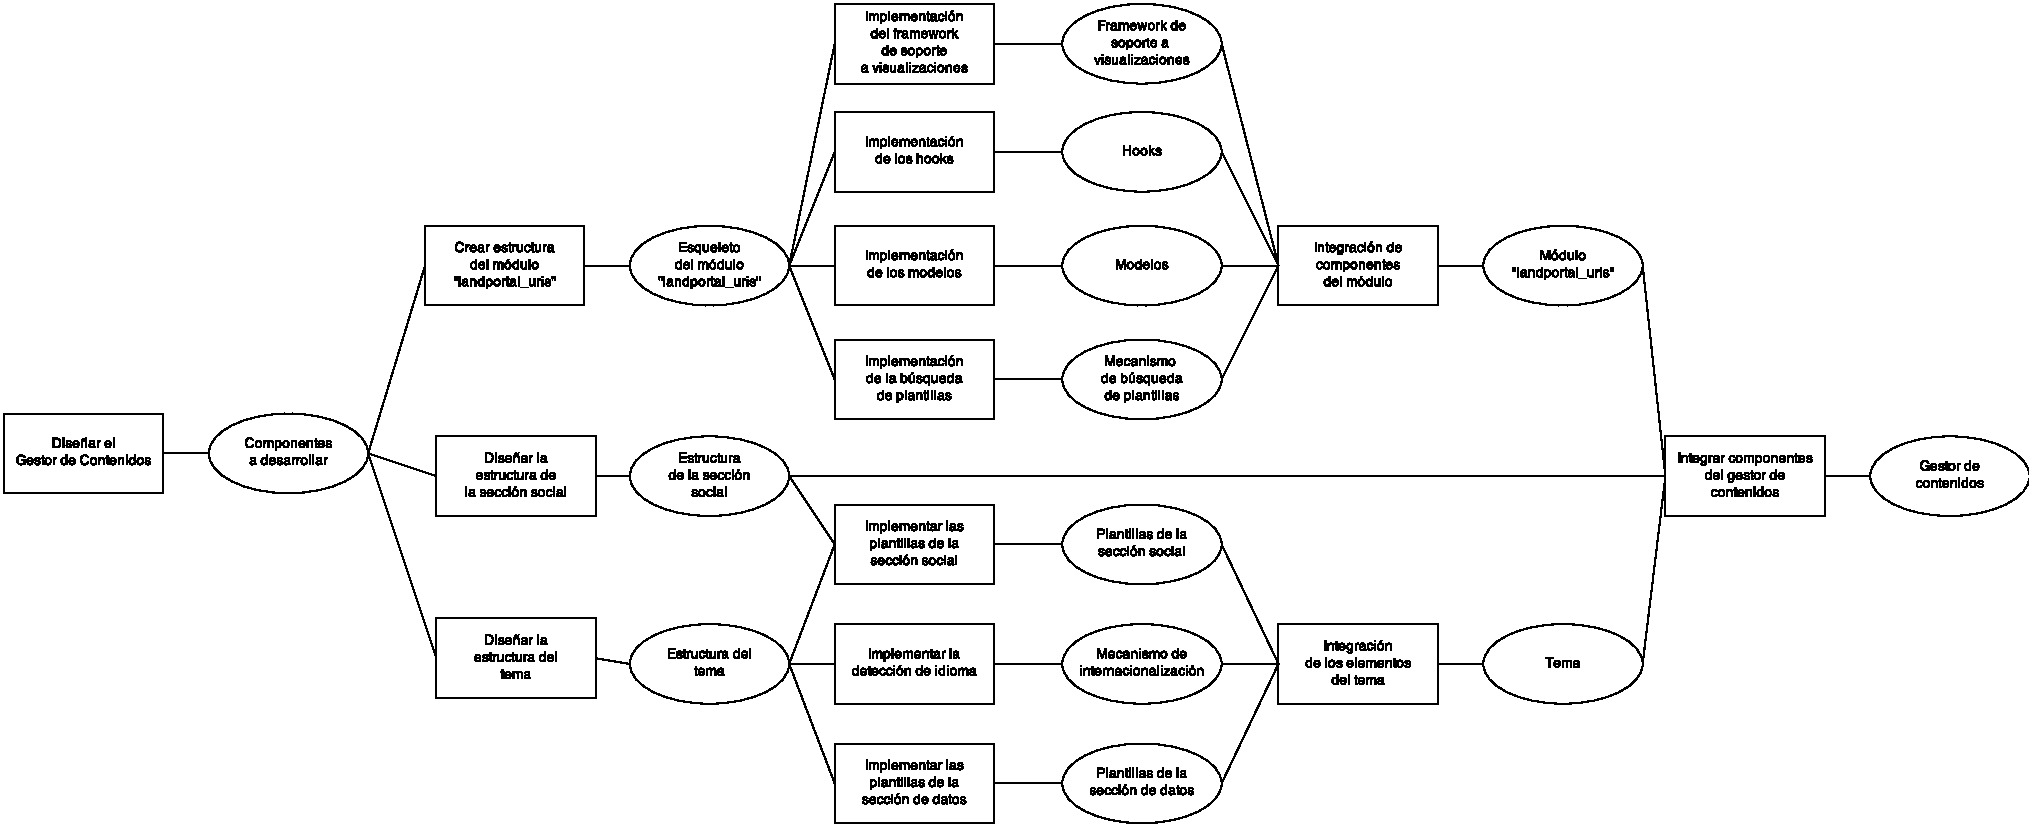
\includegraphics[width=\textwidth]{wbs/wbs_CMS}
	\caption{Estructura de desglose del trabajo del gestor de contenidos}
	\label{fig:wbs_CMS}
\end{figure}

\begin{figure}[h]
	\centering
	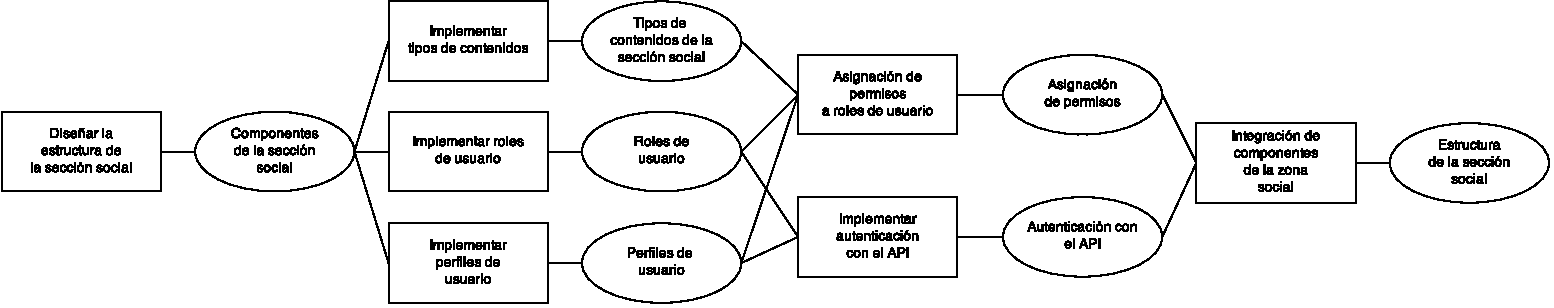
\includegraphics[width=\textwidth]{wbs/wbs_social}
	\caption{Estructura de desglose del trabajo de la fase desarrollo de la zona social}
	\label{fig:wbs_social}
\end{figure}

\begin{figure}[h]
	\centering
	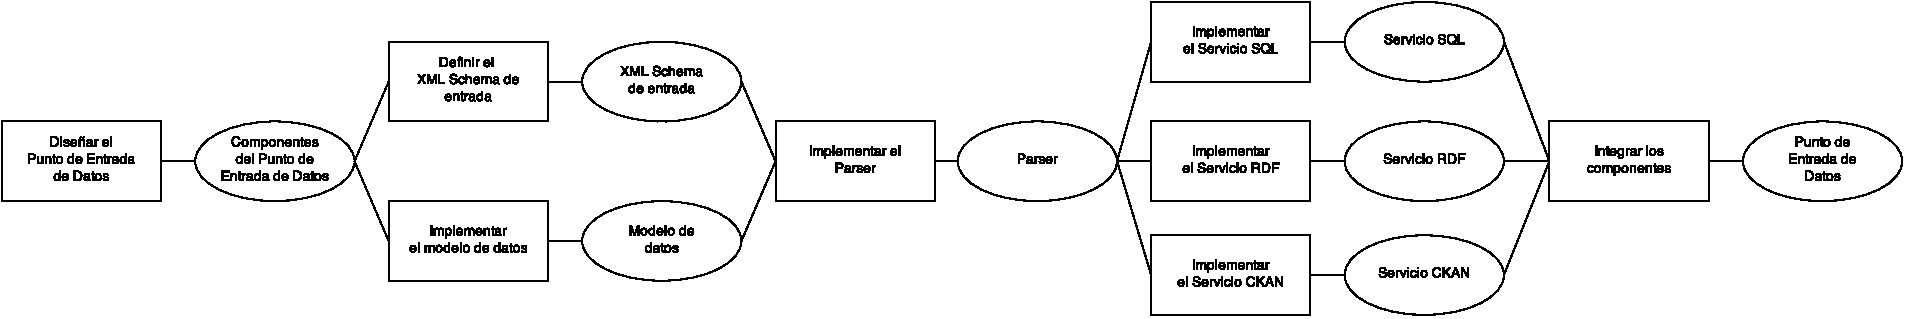
\includegraphics[width=\textwidth]{wbs/wbs_datos}
	\caption{Estructura de desglose del trabajo de la fase desarrollo del Punto de Entrada de Datos}
	\label{fig:wbs_datos}
\end{figure}

\begin{figure}[h]
	\centering
	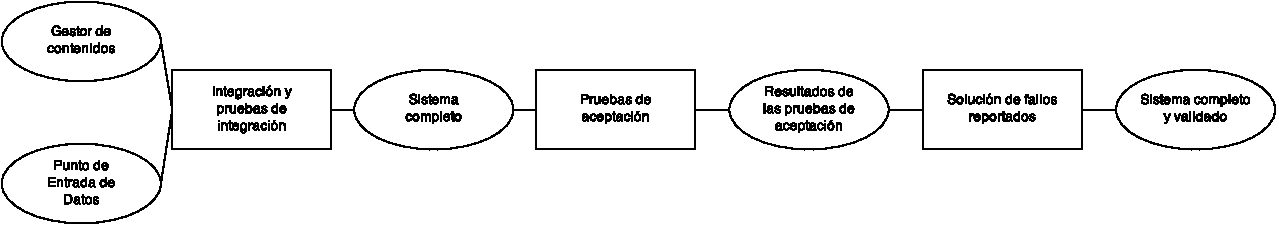
\includegraphics[width=\textwidth]{wbs/wbs_final}
	\caption{Estructura de desglose del trabajo de la fase final del sistema}
	\label{fig:wbs_final}
\end{figure}